\documentclass[../notes.tex]{subfiles}

\pagestyle{main}
\renewcommand{\chaptermark}[1]{\markboth{\chaptername\ \thechapter\ (#1)}{}}
\setcounter{chapter}{7}

\begin{document}




\chapter{Transition Metal Electronic Structure}
\section{Crystal Field Theory and Ligand Field Theory}
\begin{itemize}
    \item \marginnote{11/14:}Questions from the video lectures.
    \item For descent in symmetry questions, how do we qualitatively describe orbital energy? Do the Mulliken symbols matter?
    \begin{itemize}
        \item Rationalize based on the molecular orbital parentage.
        \begin{itemize}
            \item $a_1$ may or may not be more stable than $a_{1g}$, for example.
        \end{itemize}
        \item We need to visualize the orbitals and see if we're ripping something off from the axial or equatorial positions, for example, because that matters.
        \item The labels are just there to make sure that our molecular orbital assignments are correct within the point group. It's mainly a bookkeeping thing. It also helps us create further MOs based on symmetry, though.
        \item The Mulliken symbol alone doesn't convey any information about energetics.
    \end{itemize}
    \item Walsh diagram structure.
    \begin{itemize}
        \item Curved vs. straight lines is irrelevant; we just need to know whether the energy increases or decreases qualitatively under a procedural change in the molecule.
        \item All we need to be able to do is derive the initial and final state and know what maps to what.
    \end{itemize}
    \item How do you determine straight vs. curved line?
    \begin{itemize}
        \item No way to do this from first principles; you need a combination of DFT and experiment.
    \end{itemize}
    \item Comparing orbital energies.
    \begin{itemize}
        \item If we're deriving from a new set of orbitals (as in the \ce{FeBz} example), we need SALCs.
        \item In an exam setting, though, we won't encounter brand new orbitals.
    \end{itemize}
    \item We now start in on today's lecture topic.
    \item \textbf{CFT} and \textbf{LFT} are frameworks that help us estimate orbital energies.
    \begin{itemize}
        \item They are quantitative methods for evaluating $d$-orbital splitting.
    \end{itemize}
    \item \textbf{Crystal field theory}: A method in which one estimates ligands as point charges (which is not great, but ok) and the metal as a cation \ce{C}. \emph{Also known as} \textbf{CFT}.
    \begin{itemize}
        \item Established by physicists at the same time as the birth of inorganic chemistry, before chemists came on the scene.
        \item Ligands are structure-less and orbital-less (think like a physicist; no structure, just charge).
        \item Group theory tells us that a $d$-orbital in an $O_h$ environment has $t_{2g}$ or $e_g$ symmetry regardless of how much structure is present.
        \item Even though the transition metal \ce{C} is positive, the electrons in the $d$-orbitals are negative, so we get the following visualization.
        \item Visualization: In the free ion, you have five degenerate $d$-orbitals. You then first approximate a negatively charged spherical field around the point charge, which causes the $d$-orbitals to go-up in energy. Lastly, we split the $t_{2g}$ and $e_g$ set in an $O_h$ field. Essentially, Wuttig redraws Figure VI.11 of \textcite{bib:CHEM20100Notes}.
    \end{itemize}
    \item \textbf{Crystal field splitting parameter}: The difference in energy between the $e_g$ and $t_{2g}$ set. \emph{Denoted by} $\bm{\Delta_o}$, $\bm{10Dq}$. \emph{Also known as} \textbf{field strength}, \textbf{field splitting}.
    \begin{itemize}
        \item 10Dq nomenclature will return when we derive Tanabe-Sugano diagrams from scratch.
        \item This is a \emph{quantitative} term for the field splitting, different from every other aspect of the course this far (all of which have been qualitative).
        \item This is phenomenological parameter that is determined from experiment and cannot be calculated from first principles.
        \begin{itemize}
            \item The typical experiment is something like UV-Vis spectroscopy.
        \end{itemize}
        \item The terms field strength and field splitting are basically synonymous. However, we can also think of "field strength [as] the quantitative number associated with the field splitting."
    \end{itemize}
    \item Main takeaway of CFT: The origin of something called field splitting, and the origin of quantitatively understanding $d$-orbital energetics.
    \item We now move on from CFT to LFT.
    \item \textbf{Ligand field theory}: The same as CFT; we just put the bonds back in.
    \begin{itemize}
        \item It's not just point charges any more; there are actual bonds created by overlapping the metal $d$-orbitals (which we had also previously assumed to exist) with the ligand orbitals (which we are only adding in now).
        \item Thus, free $d$ electrons have adjustable interelectronic repulsion parameters. These are important in free ion terms.
    \end{itemize}
    \item Field splitting.
    \begin{itemize}
        \item Origins of ligand field splitting: Molecular symmetry and group theory, as discussed since the beginning of the course.
        \item Extent of ligand field splitting: We will talk about this now.
        \item Manifestations of ligand field splitting: The colors of TM complexes, reactivity, magnetism, life (bioinorganic chemistry), and many more.
    \end{itemize}
    \item There are four main things to consider when determining the magnitude of the field strength.
    \begin{enumerate}
        \item $\sigma$ and $\pi$ effects.
        \begin{itemize}
            \item We talked a bit about this when we derived the \ce{ML6} MO diagrams from scratch with and without $\pi$ orbitals.
            \begin{itemize}
                \item Recall the discussion regarding Figures \ref{fig:MOsML6}, \ref{fig:MOsML6pi}, and \ref{fig:MOsML6piAcc}.
            \end{itemize}
            \item We want to compare a $\pi$-donor, to a $\sigma$-only ligand, to a $\pi$-acceptor.
            \begin{itemize}
                \item In every case, the $e_g$ set will be comprised of \ce{M-L\sigma^*} orbitals.
                \item However, the $t_{2g}$ set will decrease in energy from \ce{M-L\pi^*} to nb to \ce{M-L\pi}, respectively.
                \item It follows that $\Delta_0$ increases as we go from $\pi$-donors, to $\sigma$-only donors, to $\pi$-acceptors.
            \end{itemize}
            \item People made this observation by looking at a series of homoleptic $O_h$ complexes, specifically the \textbf{spectrochemical series}.
        \end{itemize}
        \item Oxidation state.
        \begin{itemize}
            \item As oxidation state increases (the metal ion becomes more positive), ligand field splitting increases, too.
            \item This is because orbital overlap increases as ligands are pulled in and hence the amount of ligand field splitting increases, too.
            \begin{itemize}
                \item Mathematically, increasing the oxidation state increases the overlap integral $S$.
            \end{itemize}
            \item Alternatively, we can think of this as more electropositive transition metals drawing more electrons toward them.
            \item Wuttig illustrates this point with example $\Delta_o$ values for compounds that are alike in every way except for the oxidation state. For instance,
            \begin{align*}
                \Delta_o(\ce{Cr(H2O)6^2+}) &= \SI{14100}{\per\centi\meter}\\
                \Delta_o(\ce{Cr(H2O)6^3+}) &= \SI{17000}{\per\centi\meter}
            \end{align*}
        \end{itemize}
        \item Row of the TM on the periodic table.
        \begin{itemize}
            \item The first row has a lower field strength than the second row, which has a similar field strength to the third row.
            \item This is because the radial extension of second and third row metals is much higher, leading to better overlap (higher $S$), and thus higher splitting of bonding/anti-bonding orbitals.
            \item Example: In the following $d^6$ complexes, we can observe a drastic increase in $\Delta_o$ between the first- and second-row TM and a smaller increase in $\Delta_o$ between the second- and third-row TM.
            \begin{align*}
                \Delta_o(\ce{Co(NH3)6^3+}) &= \SI{22870}{\per\centi\meter}\\
                \Delta_o(\ce{Rh(NH3)6^3+}) &= \SI{34100}{\per\centi\meter}\\
                \Delta_o(\ce{Ir(NH3)6^3+}) &= \SI{41200}{\per\centi\meter}
            \end{align*}
        \end{itemize}
        \item Geometry.
        \begin{figure}[h!]
            \centering
            \includegraphics[width=0.5\linewidth]{../ExtFiles/geometryFieldStrength.png}
            \caption{Geometry affects field strength.}
            \label{fig:geometryFieldStrength}
        \end{figure}
        \begin{itemize}
            \item The number of ligands around the metal, as well as whether or not certain ligands are on-axis, affects the number of interactions and hence the splitting.
            \item In a $T_d$ field for example, there are far fewer on-axis repulsive interactions compared to $O_h$.
        \end{itemize}
    \end{enumerate}
    \item \textbf{Spectrochemical series}: A measure of the orbital overlap, electronegativity, and VOIE considerations that determine how big the ligand field splitting is.
    \begin{figure}[h!]
        \centering
        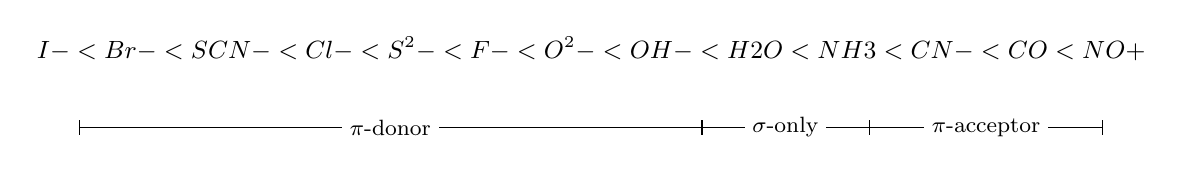
\begin{tikzpicture}[
            every node/.style={fill=white}
        ]
            \node {\small $
                \ce{I-} <
                \ce{Br-} <
                \ce{SCN-} <
                \ce{Cl-} <
                \ce{S^2-} <
                \ce{F-} <
                \ce{O^2-} <
                \ce{OH-} <
                \ce{H2O} <
                \ce{NH3} <
                \ce{CN-} <
                \ce{CO} <
                \ce{NO+}
            $};
    
            \footnotesize
            \draw [|-] (-6.5,-1) -- node{$\pi$-donor} (1.4,-1);
            \draw [|-] (1.4,-1) -- node{$\sigma$-only} (3.53,-1);
            \draw [|-|] (3.53,-1) -- node{$\pi$-acceptor} (6.5,-1);
        \end{tikzpicture}
        \caption{The spectrochemical series.}
        \label{fig:spectrochemicalSeries}
    \end{figure}
    \begin{itemize}
        \item Some ligands engender higher splitting energies than others, and we can measure this via the electronic transitions of (light absorbed/emitted by) homoleptic complexes.
        \item The spectrochemical series was initially just a qualitative observation; it was later explained by MO theory.
    \end{itemize}
    \item Example: Rationalize the following energy trends
    \begin{figure}[H]
        \centering
        \includegraphics[width=0.6\linewidth]{../ExtFiles/rowEnergyTrends.png}
        \caption{Energy trends across a row.}
        \label{fig:rowEnergyTrends}
    \end{figure}
    \begin{itemize}
        \item Trends: The \ce{M-CO} binding energy increases left to right. The orbital occupation of the \ce{CO(\pi^*)} decreases left to right. Regardless, the orbital occupation of the \ce{M($a_1$)} (primarily of $d_{z^2}$ parentage) increases left to right.
        \item The analytical procedure is as follows.
        \item Investigate the ligand: \ce{CO} is a $\pi$-acceptor; thus, the $d_{z^2}$ orbital is of \ce{M-L\sigma^*} parentage. Recall from the PES of \ce{CO} that its LUMO ($\pi^*$ symmetry) lies higher in energy than the $d$ atomic orbitals, which are sandwiched between that and the HOMO ($\sigma$ symmetry).
        \item Investigate the metal center: All molecules are third-row $d^6$ transition metals.
        \item Investigate what changes: The charge (e.g., \ce{Ir^3+} vs. \ce{Hf^2-}) and the electronegativity of the metal center (decreases left to right; does she mean the amount of negative charge?? Seems like she's been using electronegativity and electropositivity potentially wrong a few times??).
        \item On the left side, the metal $d$ orbitals are high in energy, so they are close to the high-lying \ce{CO(\pi^*)} orbitals in energy, so they donate a lot of electron density to \ce{CO(\pi^*)}. On the right side, the opposite is true.
        \item Additionally, there is a smaller gap between $d_{z^2}$ and \ce{CO(\sigma)} on the right side.
    \end{itemize}
    \item \textbf{Electronic spectroscopy}: Electron absorption spectra are broad --- occur much more rapidly than molecular vibrations, i.e., we see a snapshot of the molecule in various rotational vibrational states.
    \item We're done learning about trends and onto quantifying stuff. To understand how to quantify things better, we need to understand the origins of electronic spectra.
    \item Thus, we'll discuss some basic properties of UV-Vis spectra in relation to the Franck-Condon principle.
    \item In the first half of the course, we focused on vibration. Now we're looking at electronic excitations and, in particular, electronic excitation wells.
    \pagebreak
    \item Franck-Condon Principle.
    \begin{figure}[h!]
        \centering
        \includegraphics[width=0.3\linewidth]{../ExtFiles/FC.png}
        \caption{Franck-Condon Principle potential wells.}
        \label{fig:FC}
    \end{figure}
    \begin{itemize}
        \item $E_0$ is our ground electronic state.
        \item $E_1$ is the first electronic excited state.
        \item All of the little levels in between are the vibrational energy levels (overtones, etc.) that we discussed in the beginning.
        \item We now assume that an electronic transition is much faster than a vibrational transition, and hence occurs virtually without a change in nuclear coordinates. We just do a vertical jump from one well to the other, without moving nuclear coordinates along a vibration ("electronic transitions are `vertical' with respect to the nuclear coordinate axis").
        \item The Franck-Condon principle arises from the Born-Oppenheimer approximation.
        % \item An electronic transition is more likely to occur from the bottom to the other bottom since electronic transitions are much faster than vibrational ones. Implication: Electronic excitement or emission occurs without a change in nuclear coordinates. It's just a vertical shift/a straight arrow upwards; vibration is not really considered.
    \end{itemize}
    \item \textbf{Born-Oppenheimer approximation}: We can separate the electronic and vibrational wave functions of a given molecule.
    \item Terms next time.
\end{itemize}



\section{Electronic Spectroscopy II}
\begin{itemize}
    \item \marginnote{11/16:}No in-person lecture on Friday; a video will be posted. Watch before Monday's lecture (last lecture of the class). Wednesday is the review session, Friday is the second exam, no final.
    \item Last problem set has been posted; due the review session day. Submit virtually (as a PDF).
    \item Goal: Understand and derive term symbols in the context of electron configuration. Free ions $\to$ weak field $\to$ strong field. It's important to understand where these things come from because that allows us to use the tools in the literature in a more informed fashion.
    \item Terms allow us to predict the energy of the electronic transition. But where do they come from? How do they vary for ground and excited states?
    \item \textbf{Term}: Energy level of a spectrum.
    \item Free ion term: $d$-orbital manifold in the absence of any other geometry. We have 5 $d$ orbitals and, suppose, a $d^2$ system. We can fill electrons however we want as long as we satisfy the Pauli exclusion principle. But different fillings have different energies.
    \emph{picture}
    \item Multi-electron transition metal ions have multiple energy levels even when $d$-orbital degeneracy is not lifted by a ligand field.
    \item \textbf{Configuration}: The assignment of a given set of electrons to a certain set of orbitals.
    \begin{itemize}
        \item Applies to $d$ orbital setups that are \emph{not} free ion, i.e., degeneracy has been lifted.
        \item Each configuration gives rise to a number of energy levels and the number of energy levels have to have an even number of terms.
    \end{itemize}
    \item Example:
    \begin{itemize}
        \item 2 electrons in $d$ orbitals. $({t_{2g}}^2)$, for instance, implies that we have 2 electrons in 2 $t_{2g}$ orbitals.
        \item 4 electrons in $d$ orbitals. ${t_{2g}}^4$, for instance, implies that all electrons are in the $t_{2g}$ set. $({t_{2g}}^2)({t_{2g}}^2)$, for instance, implies that electrons are in different orbitals; this describes an excited state.
    \end{itemize}
    \item Energy ordering of the terms.
    \begin{itemize}
        \item To construct suitable energy level diagrams for various states in a transition metal ion, we consider the last three terms (IER -- interelectronic repulsion, SOC -- spin-orbit coupling, and LFI -- ligand field interaction).
        \item The interaction between these three terms determines whether we're in a weak or strong field.
        \item Case 1: $\text{IER}>\text{LFI}>\text{SOC}$ gives rise to the weak field approximation (ligand field induces only a small perturbation of the energy levels).
        \item Case 2: $\text{LFI}>\text{IER}>\text{SOC}$ gives rise to the strong field approximation (implies more low spin configurations).
    \end{itemize}
    \item We've now started understanding the underlying principles that change the energy ordering.
    \item Consider only weak field approximation. We first approximate the weakest field possible: Where there is no field. World's most boring electronic structure, but helps us understand how to build correlation diagrams. Let's determine the number of microstates or the ways we can put a single electron into $d$ orbitals.
    \begin{itemize}
        \item $d^1$ case: No effects from other electrons, yet there are still numerous microstates.
        \item A $d$ orbital can be described by $\ell=2$ (the angular momentum quantum number), $m_\ell\in\{-2,-1,0,1,2\}$ (the magnetic quantum number; takes integer values that span $-\ell$ to $\ell$), and $m_s=\pm 1/2$ (the spin quantum number).
        \item Thus, there are 5 degenerate $d$ orbitals (one for each $m_\ell$; these labels can be though of as alternatives to $z^2,x^2-y^2,\dots$).
        \item The one electron can occupy any $d$ orbital and take spin $\pm 1/2$ for 10 total degenerate sets of microstates.
        \item We can designate the collection of microstates with a term symbol.
    \end{itemize}
    \item \textbf{Term symbol}: An abbreviation describing a selection of microstates.
    \item How do I know that I need to get 10 microstates?
    \begin{itemize}
        \item The number $\ell^q$ of microstates for a given configuration, where $\ell$ is the angular momentum quantum number and $q$ is the number of electrons, can be calculated for a number of equivalent electrons. The formula is
        \begin{equation*}
            n = \frac{(4\ell+2)!}{q!(4\ell+2-q)!}\footnotemark
        \end{equation*}
        \footnotetext{Wuttig puts $4\ell-2$ in the denominator.}
        \item If we do this for $\ell=2$, $q=1$, we get
        \begin{equation*}
            n = \frac{10!}{9!} = 10
        \end{equation*}
    \end{itemize}
    \item How do I know what the term symbol is?
    \begin{itemize}
        \item Term symbols have the form ${}^{2S+1}L_J$.
        \item $M_L=\sum m_\ell$ for a given microstate.
        \item $M_S=\sum m_s$ for a given microstate.
        \item $S$, the spin multiplicity, is the total spin angular momentum (values $0,1/2,1,3/2,2,5/2$) or the maximum $M_S$ value.
        \item $L$, the total orbital angular momentum, is the maximum $M_L$ value.
        \item $J$, the L-S/Russell-Saunders/spin-orbit coupling, is only relevant for multielectron systems where the presence of an electron in the same shell diminishes the coupling of another. $J$ is the total angular momentum. $J=L+S,L+S-1,L+S-2,\dots,L-S-1,L-S$\footnote{This is probably wrong, too; should iterate down to $|L-S|$.}.
    \end{itemize}
    \item Example: Term symbol for $d^1$.
    \begin{itemize}
        \item We must have $S=1/2$ (the smallest possible value of $S$, and the only one achievable by one electron) and $L=2$ (degenerate set of orbitals that span $-2$ to 2). Thus, ${}^2D$.
        \item No spin-orbit coupling to worry about because there's only one electron in the system (coupling inherently requires two or more electrons).
    \end{itemize}
    \item Multielectron atom procedure.
    \begin{enumerate}
        \item Determine the total number of microstates ($m_\ell$, $m_s$ values).
        \item Determine the possible values of $M_L=\sum m_\ell$ and $M_S=\sum m_s$.
        \item Construct a Pauli-allowed chart of microstates.
        \item Group microstates into terms.
        \item Assign ground state term symbol.
    \end{enumerate}
    \item Let's tackle $d^2$.
    \begin{itemize}
        \item By the formula, there are 45 microstates.
        \item Goes through the microstate table and rectangles (we won't be asked to derive this, though).
        \item The maximum value of $L$ is 4. This means the two electrons are in the same orbital, so we have $S=0$. Thus, we get ${}^1G$ for our term symbol. We now slash off all microstates for which $L=4$ and $S=0$, i.e., microstates for which $M_L=0,\pm 1,\pm 2,\pm 3,\pm 4$ and $M_S=0$.
        \item Next up is $L=3$ for maximum possible $L$. Maximum possible $S$ in this case is 1. Thus, we slash off all states for which $M_L=0,\pm 1,\pm 2,\pm 3$ and $M_S=0,\pm 1$ except the ones we've already counted\footnote{Note that since there are $7=2L+1$ possible $M_L$ values and $3=2S+1$ possible $M_S$ values, we will have $7\cdot 3=21$ microstates of this type. This is where Talapin's $(2L+1)(2S+1)$ formula comes from!}. Now that we have $L=3$, the electrons can be in different orbitals, so $S=1$.
        \item My big question: What do the microstates that we group together into one term symbol have in common??
    \end{itemize}
    \item Takeaway: We have multiple term symbols/energy levels for free ion states.
    \item For $d^2$, we show in handout that we have 5 terms:
    \begin{align*}
        {}^1S&&
        {}^3P&&
        {}^1D&&
        {}^3F&&
        {}^1G
    \end{align*}
    \item But how do we order the energy? Use Hund's rules:
    \begin{enumerate}
        \item Maximize the spin multiplicity (i.e., terms with higher multiplicity will have lower energy).
        \item Maximize the total angular momentum (i.e., terms with higher $L$ will have lower energy).
    \end{enumerate}
    \item Thus, the energy ordering is ${}^3F,{}^3P,{}^1G,{}^1D,{}^1S$.
    \item Electron hole formalism: $d^n$ and $d^{10-n}$ have equivalent weak field energy orderings.
    \begin{itemize}
        \item Will be asked about in our homework.
    \end{itemize}
\end{itemize}




\end{document}